\documentclass[a4paper, 10pt, ngerman]{article}
\usepackage{tikz-network}
\usepackage[left=3.5cm, right = 3.5cm, top=3.5cm, bottom=3.5cm, head=13.6pt]{geometry}
\usepackage{babel}
\usepackage[T1]{fontenc}
\usepackage{inputenc}
\usepackage[noend,nosemicolon,algoruled,noline]{algorithm2e}
\usepackage{amsmath}
\usepackage{amsthm}
\usepackage[nottoc,notlot,notlof]{tocbibind}
\usepackage{graphicx}
\usepackage{float}
\usepackage{enumitem}
\usepackage{listings}
\usepackage{color}
\usepackage{booktabs}
\usepackage{hyperref}
\usepackage{minted}
\usepackage[inkscapeformat=pdf]{svg}

\newcommand{\Aufgabe}{Aufgabe 1: Weniger krumme Touren}
\newcommand{\TeilnahmeId}{67571}
\newcommand{\Name}{Finn Rudolph}

\usepackage{scrlayer-scrpage, lastpage}
\setkomafont{pageheadfoot}{\textrm}
\rohead{Teilnahme-ID: \TeilnahmeId}
\lohead{\Aufgabe}
\cfoot*{\thepage{}}

\title{\LARGE \textbf{\Aufgabe}}
\author{\large Finn Rudolph \\ \\ \large Teilnahme-ID: 67571}
\date{\large 18. März 2022}

\setlist[enumerate]{label*={\arabic*.}}

\definecolor{keyword}{rgb}{0.2, 0.0, 0.7}
\definecolor{comment}{rgb}{0.5, 0.5, 0.5}
\definecolor{number}{rgb}{0.5, 0.5, 0.5}
\definecolor{string}{rgb}{0.3, 0.65, 0.0}

\lstset
{
    basicstyle=\footnotesize\ttfamily,
    keywordstyle=\color{keyword},
    commentstyle=\color{comment},
    numberstyle=\tiny\color{number},
    stringstyle=\color{string},
    numbers=left,
    showspaces=false,
    showstringspaces=false
}

\hypersetup
{
    colorlinks=true, 
    urlcolor=blue, 
    linkcolor=black, 
    citecolor=black, 
    pdftitle={Aufgabe 1: Weniger krumme Touren}
}

\begin{document}

\begin{titlepage}
    \maketitle
    \tableofcontents
    \thispagestyle{empty}
\end{titlepage}

\newtheorem{theorem}{Satz}
\newtheorem{lemma}{Lemma}
\theoremstyle{definition}
\newtheorem{definition}{Definition}

\section{Lösungsidee}

Das Problem wird durch einen Graphen modelliert. Jeder Punkt wird einem Knoten zugeordnet und zwischen jedem Knotenpaar existiert eine ungerichtete Kante, deren Gewicht die euklidsche Distanz zwischen den zugehörigen Punkten ist. Das Ziel ist es, einen möglichst kurzen Hamiltonpfad durch diesen Graphen zu finden. Die Bedingung, dass kein Abbiegewinkel von mehr als 90° vorkommen darf, bedeutet, dass bestimmte Tripel an Knoten nicht direkt aufeinander folgen dürfen. Das Problem soll als ganzzahliges lineares Programm (IP) formuliert werden und mithilfe eines IP-Solvers gelöst werden. Da es NP-schwer ist, wie später gezeigt wird, ist es unwahrscheinlich, dass ein Algorithmus mit polynomieller Laufzeit 

\subsection{Formulierung als ganzzahliges lineares Programm}

Im Folgenden wird mit $d_{ij}$ die euklidsche Distanz zwischen Punkt $i$ und Punkt $j$, für $0 \le i, j \le n - 1$ bezeichnet, wobei $n$ die Anzahl an Punkten ist. Daneben bezeichnet $\vec{z_i}$ den zweidimensionalen Ortsvektor zu Punkt $i$. $\vec{z_{ij}}$ bezeichnet den Vektor $\vec{z_j} - \vec{z_i}$. Der beschriebene Graph heißt $G = (V, E)$, mit Knotenmenge $V$ und Kantenmenge $E$. Für die IP-Formulierung definieren wir die binären Variablen $x_{ij}$ für $0 \le i, j \le n - 1, i < j$, sodass $x_{ij} = 1$, wenn die Kante zwischen Punkt $i$ und Punkt $j$ in der optimalen Lösung verwendet wird, andernfalls $x_{ij} = 0$. Die Einschränkung $i < j$ ist sinnvoll, um die Anzahl nötiger Variablen zu halbieren. Im Folgenden wird der Einfachheit halber manchmal $x_{ij}$ auch für $i > j$ geschrieben, gemeint ist dann immer $x_{ji}$. Das ganzzahlige lineare Programm sieht wie folgt aus.

\begin{align*}
    \text{minimiere} \quad & \sum_{i = 0}^{n - 1} \sum_{j = i + 1}^{n - 1} x_{ij} d_{ij} & & \quad (1) \\
    \text{sodass} \quad 
    & \sum_{j = 0, j \ne i}^{n - 1} x_{ij} \ge 1 & 0 \le i \le n - 1 & \quad (2) \\
    & \sum_{j = 0, j \ne i}^{n - 1} x_{ij} \le 2 & 0 \le i \le n - 1 & \quad (3) \\
    & \sum_{i = 0}^{n - 1} \sum_{j = i + 1}^{n - 1} x_{ij} = n - 1 & & \quad (4) \\
    & \sum_{i \in S} \sum_{j \in S, i < j} x_{ij} \le |S| - 1 & S \subseteq V, S \ne \emptyset & \quad (5) \\
    & x_{ij} + x_{jk} \le 1 & 0 \le i, j, k \le n - 1, i \ne j \ne k, i < k, \vec{z_{ij}} \cdot \vec{z_{jk}} < 0 & \quad (6) \\
    & x_{ij} \in \{0, 1\} & 0 \le i, j \le n - 1, i < j & \quad (7)
\end{align*}
\smallskip

In der Zielfunktion (1) werden die Längen aller verwendeten Kanten summiert. Ungleichungen (2) und (3) beschränken den Grad jedes Knoten auf 1 oder 2. Gleichung (4) sorgt dafür, dass insgesamt $n - 1$ Kanten verwendet werden. Ungleichung (5) ist der \emph{Subtour Elimination Constraint (SEC)} in der Formulierung von Dantzig, Fulkerson und Johnson (DFJ) \cite{tsp-formulations}, durch den die Konnektivität des Pfads sichergestellt wird. Ungleichung (6) setzt die Einschränkung des Abbiegewinkels um, wobei $\cdot$ das Skalarprodukt bezeichnet. Es wird nun gezeigt, dass die Lösung des IPs in (1) - (7) einen kürzesten Hamiltonpfad mit Abbiegewinkeln kleiner gleich $\pi / 2$ bildet. 

Wir nennen einen Hamiltonpfad mit Abbiegewinkeln kleiner gleich $\pi / 2$ auch einen \emph{zulässigen Pfad}. Damit von dem linearen Programm der kürzeste zulässige Pfad gefunden wird, muss die Menge zulässiger Pfade genau mit der Menge an Pfaden, die durch Gleichungen (2) - (7) erlaubt sind, übereinstimmen. Denn dann wird durch die Zielfunktion in (1) der kürzeste von ihnen gewählt. Zunächst wird gezeigt, dass jeder Pfad, der die Gleichungen (2) - (7) erfüllt, zulässig ist. Dafür sei $X = \{\{i, j\} : x_{ij} = 1\}$ die Menge an Kanten, die in der Lösung des ganzzahligen linearen Programms verwendet werden.

\begin{lemma}
    Der Graph $G' = (V, X)$ enthält keine Zyklen.
\end{lemma}

\begin{proof}
    Für einen Widerspruch nehme man an, dass sich ein Zyklus in $G'$ befindet, der genau die Knoten der Menge $T$ enthält. Dann gilt
    \begin{align*}
        \sum_{i \in T} \sum_{j \in T, i < j} x_{ij} \ge |T|
    \end{align*}
    da ein Zyklus aus $|T|$ Knoten genau $|T|$ Kanten enthält. Das ist ein Widerspruch zu (5) mit $S = T$, folglich war die Annahme, dass $G'$ einen Zyklus enthält, falsch.
\end{proof}

\begin{lemma}
    Die Kanten in $X$ bilden einen Hamiltonpfad in $G$.
\end{lemma}

\begin{proof}
    Wegen (4) enthält $G' = (V, X)$ genau $n - 1$ Kanten und wegen Lemma 1 ist $G'$ azyklisch. Ein azyklischer Graph mit $n - 1$ Kanten ist ein Baum mit $n$ Knoten, und damit ist $G'$ ein Spannbaum von $G$. Da der Grad jedes Knoten von (3) auf maximal 2 begrenzt wird, hat $G'$ genau zwei Blätter. Wählt man diese beiden Blätter als Endpunkte eines Pfads in $G$, erhält man einen Hamiltonpfad.
\end{proof}
 
Ungleichung (2) ist zur Sicherstellung der gewünschten Eigenschaften von $X$ nicht nötig, verkürzte jedoch praktisch die Laufzeit, weshalb sie mit aufgeführt ist.

\begin{lemma}
    Jeder Abbiegewinkel zwischen zwei aneinanderliegenden Kanten in $X$ ist kleiner oder gleich $\pi / 2$.
\end{lemma}

\begin{proof}
    Der Abbiegewinkel $\alpha$ zweier Vektoren $\vec{u}$ und $\vec{v}$ ist der Betrag des Außenwinkels $\gamma$ zwischen ihnen. Der Außenwinkel ist mit dem Skalarprodukt durch folgende Identität verknüpft.
    \begin{align*}
        \cos(\gamma) = \frac {\vec{u} \cdot \vec{v}} {|\vec{u}||\vec{v}|}
    \end{align*}
    Da $|\gamma| \le \pi / 2 \Longleftrightarrow \cos(\gamma) \ge 0$ und $|\vec{u}| |\vec{v}| \ge 0$, ist $|\gamma| \le \pi / 2$ äquivalent zu $\vec{u} \cdot \vec{v} \ge 0$. Für einen Widerspruch nehme man an, dass der Betrag des Außenwinkels zwischen zwei unterschiedlichen Kanten $\{i, j\} \in X$ und $\{j, k\} \in X$ größer als $\pi / 2$ ist. Da die Kanten unterschiedlich sind, gilt $i \ne j \ne k$. Es wird außerdem angenommen, dass $i < k$, was durch Tauschen von $i$ und $k$ immer erreicht werden kann. Dann gilt $x_{ij} + x_{jk} = 2$ und $\vec{z_{ij}} \cdot \vec{z_{jk}} < 0$, ein Widerspruch zu (6). 
\end{proof}

Die Einschränkung $i < k$ in Ungleichung (6) ist nicht notwendig, sie könnte auch durch $i \ne k$ ersetzt werden, wodurch jedoch Dopplungen entstehen würden. Aus Lemma 2 und 3 folgt, direkt, dass jeder Pfad, der von (2) - (7) erlaubt wird, zulässig ist. Nun gilt es noch, die Umkehrung zu zeigen, dass jeder zulässige Pfad (2) - (7) erfüllt. (Das ist nötig, da es sonst einen kürzesten zulässigen Pfad geben könnte, der durch (2) - (7) fälschlicherweise ausgeschlossen wird.) Ungleichung (7) muss gelten, da eine Kante entweder im Pfad enthalten oder nicht enthalten ist.

\begin{lemma}
    Jeder zulässige Pfad erfüllt die Gleichungen bzw. Ungleichungen (2) - (4).
\end{lemma}

\begin{proof}
    In einem Hamiltonpfad muss jeder Knoten mindestens eine angrenzende Kante haben, da der Pfad sonst nicht jeden Knoten besuchen würde. Außerdem kann kein Knoten mehr als zwei angrenzende Kanten haben, da in einem Hamiltonpfad kein Knoten zweimal besucht wird. Gleichung (4) ist erfüllt, da ein Hamiltonpfad aus $n$ Knoten besteht, und ein einfacher Pfad mit $n$ Knoten $n - 1$ Kanten besitzt.
\end{proof}

\begin{lemma}
    Jeder zulässige Pfad erfüllt Ungleichung (5).
\end{lemma}

\begin{proof}
    Wäre Ungleichung (5) nicht erfüllt, könnte man eine Menge an Knoten $T$ wählen, zwischen denen mindestens $|T|$ Kanten des Pfades verlaufen. Dadurch wird zwingend ein Zyklus in $T$ geschaffen, ein Widerspruch dazu, dass die betrachteten Kanten Teil eines Hamiltonpfades sind.
\end{proof}

\begin{lemma}
    Jeder zulässige Pfad erfüllt Ungleichung (6).
\end{lemma}

\begin{proof}
    Wenn Ungleichung (6) nicht erfüllt ist, gibt es drei Knoten $i, j, k$, sodass $i \ne j \ne k$, $i < k$, $\vec{z_{ij}} \cdot \vec{z_{jk}} < 0$ und sowohl $x_{ij} = 1$ als auch $x_{jk} = 1$. Das heißt, sowohl die Kante $\{i, j\}$ als auch die Kante $\{j, k\}$ liegt auf dem Pfad (und $\{i, j\} \ne \{j, k\}$) und das Skalarprodukt ihrer zugehörigen Vektoren ist negativ. Wie in Lemma 3 aber bereits gezeigt wurde, ist ein negatives Skalarprodukt gleichwertig zu einem Abbiegewinkel größer $\pi / 2$, was der Annahme widerspricht, dass der betrachtete Pfad zulässig ist.
\end{proof}

\begin{theorem}
    Die Lösung des ganzzahligen linearen Programms in (1) - (7) ist ein kürzester zulässiger Pfad. 
\end{theorem}

\begin{proof}
    Folgt direkt aus den Lemmata 1 - 6 und der Minimierung der Gesamtlänge des Pfads durch (1).
\end{proof}

\emph{Anmerkungen.} 
\begin{itemize}
    \item Im Allgemeinen muss das IP in (1) - (7) keine Lösung besitzen. Ein Gegenbeispiel ist jedes Dreieck, dass keinen Winkel größer oder gleich $\pi / 2$ besitzt.
    \item Für jedes ungeordnete Tripel an Punkten $\{i, j, k\}$ werden von (6) drei Bedingungen hinzugefügt, wenn das Dreieck $ijk$ spitzwinklig ist, andernfalls zwei Bedingungen. Im Fall eines spitzwinkligen Dreiecks könnte man die drei Bedingungen auch durch eine ersetzen, nämlich $x_{ij} + x_{jk} + x_{ki} \le 1$. Obwohl diese Bedingung stärker als die drei einzelnen ist, wurde die Laufzeit nach einer Ersetzung verschlechtert.
\end{itemize} 

\subsection{Allmähliches Hinzufügen von Subtour Elimination Constraints}

Die Anzahl an Bedingungen aus (5) beträgt $2^n - 1$, da für jede nichtleere Teilmenge von $V$ ein SEC hinzugefügt wird. Das ist bereits für moderate Eingabegrößen nicht mehr praktikabel, weshalb folgendes Verfahren verwendet wird. Zu Beginn werden die SECs weggelassen und das IP optimal gelöst. Befinden sich in der Lösung Zyklen, wird für jede Knotenmenge, die in der Lösung einen Zyklus bildet, ein SEC hinzugefügt und das Verfahren wiederholt, bis die Lösung keine Zyklen mehr enthält. Das ist der übliche Weg, wie die DFJ-Formulierung von Subtour Elimination Constraints verwendet wird \cite{tsp-formulations}. Die DFJ-Formulierung wurde ursprünglich für das Problem des Handlungsreisenden (TSP) entwickelt.

In \cite{tsp-formulations} finden sich noch viele andere Möglichkeiten zur Formulierung von Subtour Elimination Constraints für das TSP, von denen die meisten auch auf dieses Problem übertragbar sind. Da viele von diesen für das TSP sowohl theoretisch als auch praktisch effizienter als die DFJ-Formulierung sind, soll begründet werden, warum sie dennoch gewählt wurde. Durch die Einschränkung des Abbiegewinkels werden bereits einige Subtouren eliminiert, z. B. alle mit 2 oder 3 Knoten, alle mit 4 Knoten, die kein Rechteck bilden, und allgemein alle, die mindestens einen Abbiegewinkel größer $\pi / 2$ haben. Für all diese Subtouren sind SECs redundant, weshalb bei diesem Problem meistens schon nach wenigen Iterationen des beschriebenen Verfahrens genügend SECs vorhanden sind. Bei anderen Formulierungen wird dagegen die Komplexität des IP durch zusätzliche Variablen erhöht, da für jede andere Formulierung mindestens $\Theta(n^2)$ zusätzliche Variablen nötig sind. Dafür ist bei diesen nur eine einzige Lösung des IPs nötig. Mit der DFJ-Formulierung kann die Laufzeit aber insgesamt geringer sein, da in jeder Iteration ein deutlich kleineres IP gelöst werden muss, und aufgrund der Winkelbeschränkungen nur wenige Iterationen nötig sind. Diese Begründung konnte experimentell unterstützt werden, siehe den Abschnitt Beispiele.

\subsection{Heuristische Lösung für große Instanzen}

Mithilfe eines IP-Solvers und der obigen Formulierung konnten alle Instanzen von BWINF optimal gelöst werden. Größere Instanzen als lin318 (318 Knoten) von TSPLIB \cite{tsplib} konnten aufgrund der zu hohen Laufzeit und des zu hohen Speicherverbrauchs aber nicht gelöst werden. Daher soll noch ein heuristisches Verfahren, basierend auf dem randomisierten Algorithmus zum Finden von Hamiltonzyklen von Posá vorgestellt werden. Mit ihm war es möglich, einen zulässigen Pfad für die Instanz pla85900 (85900 Knoten) von TSPLIB zu finden. 

Der Algorithmus funktioniert wie folgt: Zuerst wird ein zufälliger Startknoten ausgewählt. Anschließend wird ein zufälliger Knoten gewählt, der noch nicht im Pfad ist und vom letzten Knoten erreichbar ist, ohne dass ein Abbiegewinkel kleiner $\pi / 2$ entsteht. Existiert kein solcher Knoten, wird das Ende des Pfads als Sackgasse markiert und versucht, das andere Ende auf die gleiche Weise zu erweitern. Sind beide Enden des Pfads als Sackgasse markiert, wird eine zufällige Kante aus dem Pfad ausgewählt und entfernt. Anschließend wird der Knoten am hinteren Ende des Pfads so mit einem der Endpunkte der entfernten Kante verbunden, dass der Pfad wieder verbunden ist. Natürlich werden bei der zufälligen Wahl der Kante nur solche Kanten in Betracht gezogen, dass die neu eingefügte Kante vom Knoten am Ende des Pfads nicht die Beschränkung des Abbiegewinkels verletzt. Existiert keine solche Kante, wird das gleiche mit dem Knoten am vorderen Ende des Pfads versucht. Dem Pfad eine Richtung zu geben, auch wenn er eigentlich ungerichtet ist, ist für die Implementierung nötig und erlaubt präzisere Beschreibungen. Durch Aufbrechen des Pfads und neues Verbinden des ersten oder letzten Knotens kann der Pfad anschließend häufig erweitert werden. Die beschriebene Operation wird im Folgenden \emph{Neuverbindung} genannt. Es kann aber vorkommen, dass weder eine Neuverbindung des ersten noch des letzten Knotens möglich ist, oder dass sich die gleichen Neuverbindungen in eine Zyklus immer wieder abwechseln. Durch eine zufällige Wahl der entfernten Kante kann das meistens verhindert werden, aber nicht immer. Für diesen Fall wird eine Oberschranke an aufeinanderfolgenden Neuverbindungen festgelegt. Wird diese überschritten, wird die gesamte Suche von neuem gestartet.

Das Verfahren ist im Algorithmus \textsc{RandomizedObtusePath} zusammengefasst. $z$ enthält die Ortsvektoren aller Punkte, sodass $\vec z_i$ der Ortsvektor des $i$-ten Punkts, wie oben definiert, ist. \emph{path} enthält die Knoten des aktuellen Pfads in Reihenfolge, \emph{noAddedNode} ist der Zähler für die Anzahl konsekutiver Neuverbindungen (oder, äquivalent, der Anzahl an Ausführungen der while-Schleife, in denen kein Knoten zu \emph{path} hinzugefügt wurde). In der while-Schleife wird zunächst geprüft, ob das Limit von \emph{noAddedNode} überschritten wurde, wobei sich $n/2$ experimentell als guter Wert herausgestellt hat. Ein zu großes Limit sorgt für eine größere Laufzeit, wenn ein ohnehin aussichtsloser Pfad noch lange versucht wird, zu erweitern, mit einem zu kleinen Limit wird die Suche dagegen sehr schnell abgebrochen, obwohl eine Erweiterung noch möglich gewesen wäre. Denn manchmal ist eine längere Folge an Neuverbindungen nötig, um den Pfad wieder erweiterbar zu machen. $w$ bezeichnet den Knoten, der als nächstes an den Pfad angehängt werden soll. Anschließend wird über jeden noch nicht besuchten Knoten $x$ iteriert, und wenn das Anhängen eines Knotens einen Abbiegewinkel kleiner gleich $\pi / 2$ erzeugt, d. h. $\vec z_{vu} \cdot \vec z_{ux} \ge 0$, wird $x$ als Kandidat zur Erweiterung in Betracht gezogen. Dazu wird zunächst die Anzahl an Kandidaten erhöht, und anschließend $w$ mit Wahrscheinlichkeit $1 / \emph{candidates}$ auf $x$ gesetzt. Dass damit jeder mögliche Kandidat mit gleicher Wahrscheinlichkeit gewählt wird, lässt sich durch einen simplen Beweis durch Induktion zeigen: Für einen Kandidaten stimmt die Aussage trivialerweise, und wenn der $k$-te Kandidat betrachtet wird, hat er eine Wahrscheinlichkeit von $1/k$, $w$ zu werden, und jeder andere $1/(k-1) \cdot (k - 1) / k = 1 / k$. Wenn $w$ nach der for-Schleife nicht nil ist, wird der Pfad erweitert und die nächste Iteration der while-Schleife gestartet, andernfalls wird das hintere Ende als Sackgasse markiert. Wenn nicht beide Enden Sackgassen sind, wird der Pfad umgekehrt, um eine Erweiterung vom anderen Ende zu versuchen (unter dem letzten \textbf{else}). Andernfalls wird versucht, eine Kante im Pfad zu entfernen und $u$ mit einem ihrer Endpunkte zu verbinden. Dazu wird über alle Knoten außer den zwei letzten in \emph{path} iteriert und geprüft, ob die Kante von $u$ zum $i$-ten Knoten in \emph{path} unter Beachtung der Einschränkung des Abbiegewinkels eingefügt werden kann. Aus allen Knoten, bei denen das möglich ist, wird einer mit dem gleichen Verfahren wie oben zufällig ausgewählt (wieder $w$ genannt). Wenn $w$ nach Ende der for-Schleife nicht nil ist, wird $u$ mit $w$ ,,verbunden'', indem das Suffix von \emph{path} nach $w$ umgekehrt wird, so sind $u$ und $w$ in \emph{path} benachbart. Existiert kein solches $w$, wird der gesamte Pfad umgekehrt, um das gleiche Verfahren für die andere Seite zu wiederholen.

\begin{algorithm}
    \emph{path} $\gets [\text{random integer between 0 and $n - 1$}]$ \; 
    \emph{noAddedNode} $\gets$ 0 \;
    \emph{frontIsDeadEnd} $\gets$ \textbf{false}, \emph{backIsDeadEnd}  $\gets$ \textbf{false}\;

    \While{path.length $< n$}
    {
        \If{noAddedNode $> n/2$}
        {
            reset \emph{path, noAddedNode, frontIsDeadEnd, backIsDeadEnd} and restart \;
        }
        $u \gets$ last element of \emph{path}, $v \gets$ second last element of path \;
        $w \gets$ nil; \;
        \emph{candidates} $\gets$ 0 \;

        \For{\emph{node} $x \notin \text{path}$}
        {
            \If{$\vec z_{vu} \cdot \vec z_{ux} \ge 0$}
            {
                \emph{candidates} $\gets \emph{candidates} + 1$ \;
                $w \gets x$ with probability $1 / \emph{candidates}$ \;
            }
        }
        \If{$w \ne \mathrm{nil}$}
        {
            append $v$ at the back of \emph{path} \;
            \emph{noAddedNode} = 0 \;
            \textbf{continue} \;
        }

        \emph{noAddedNode} $\gets$ $\emph{noAddedNode} + 1$ \;
        \emph{backIsDeadEnd} $\gets$ \textbf{true} \;

        \If{frontIsDeadEnd \emph{\textbf{and}} backIsDeadEnd}
        {
            \emph{candidates} $\gets 0$ \;
            $w \gets$ nil \;

            \For{$i \gets \emph{path.length} - 3$ \KwTo $0$}
            {
                \If{$\vec z_{vu} \cdot \vec z_{u,\text{path}[i]} \ge 0$ \emph{\textbf{and}} $\vec z_{u,\text{path}[i]} \cdot \vec z_{\text{path}[i], \text{path}[i - 1]} \ge 0$}
                {
                    \emph{candidates} $\gets \emph{candidates} + 1$ \;
                    $w \gets$ \emph{path}$[i]$ with probability $1 / \emph{candidates}$ \;
                }
            }

            \If{$w \ne \emph{nil}$}
            {
                reverse the suffix of \emph{path} starting at the node after $w$ \;
                \emph{backIsDeadEnd} $\gets$ \textbf{false} \;
            } \Else {
                reverse \emph{path} \;
            }
        } \Else {
            reverse \emph{path} \;  
            exchange \emph{frontIsDeadEnd} with \emph{backIsDeadEnd} \;
        }

    }

    \Return{\emph{points in $z$ in the permutation stored in \emph{path}}}

    \caption{\textsc{RandomizedObtusePath}(z)}
\end{algorithm}

\textsc{RandomizedObtusePath} ist zwar in der Lage, für große Instanzen zulässige Pfade zu finden, achtet aber in keiner Weise auf deren Länge. Daher wird nach der Ausführung von \textsc{RandomizedObtusePath} noch die 2-opt Heuristik (unter Beachtung der Abbiegewinkel) verwendet, um die Länge des Pfads zu reduzieren. Die Idee der 2-opt Heuristik ist die Folgende: Solange es ein Kantenpaar gibt, sodass eine Vertauschung zweier Endknoten von diesem (also z. B. $\{u, v\}, \{x, y\}$ wird durch $\{u, x\}, \{v, y\}$ ersetzt) zu einem kürzeren Pfad führt, vertausche die Endknoten. Dabei wird natürlich darauf geachtet, keinen Zyklus und keine Abbiegewinkel größer $\pi / 2$ zu kreieren.

\section{Beweis der NP-Schwere}

Von dem nah verwandten Problem, einen Hamiltonzyklus mit einer Einschränkung des  Abbiegewinkels zu finden, wurde die NP-Schwere von Dumitrescu und Jiang \cite{nphard} bereits bewiesen. Dieses Problem wird dort \emph{Angle-bounded Hamiltonian Tour} genannt, analog wird das hier vorliegende \emph{Angle-bounded Hamiltonian Path} genannt. Der Beweis für Hamiltonpfade sieht ähnlich aus und wird hier auf Basis des Beweises in \cite{nphard} gezeigt. In \cite{nphard} wurde das NP-schwere Problem, eine Menge an Punkten im zweidimensionalen Raum mit möglichst wenigen Geraden abzudecken (\emph{Covering points by lines}) auf \emph{Angle-bounded Hamiltonian Tour} reduziert. Sei $P$ die Punktemenge der Instanz von \emph{Covering points by lines}. Zunächst wird eine Gerade durch jedes Paar an unterschiedlichen Punkten in $P$ gelegt, wobei man annehmen kann, dass keine Gerade vertikal verläuft, da man die Punkte einfach leicht rotieren könnte. Diese Menge an Geraden wird $L_P$ genannt. Anschließend wird eine Kurve $\gamma$ wie in Abbildung 1 zu sehen um $P$ herumgelegt, wobei für jede Gerade aus $L_P$ ein kleines Segment auf der linken und rechten Seite eingefügt wird.

\begin{figure}[h]
    \centering
    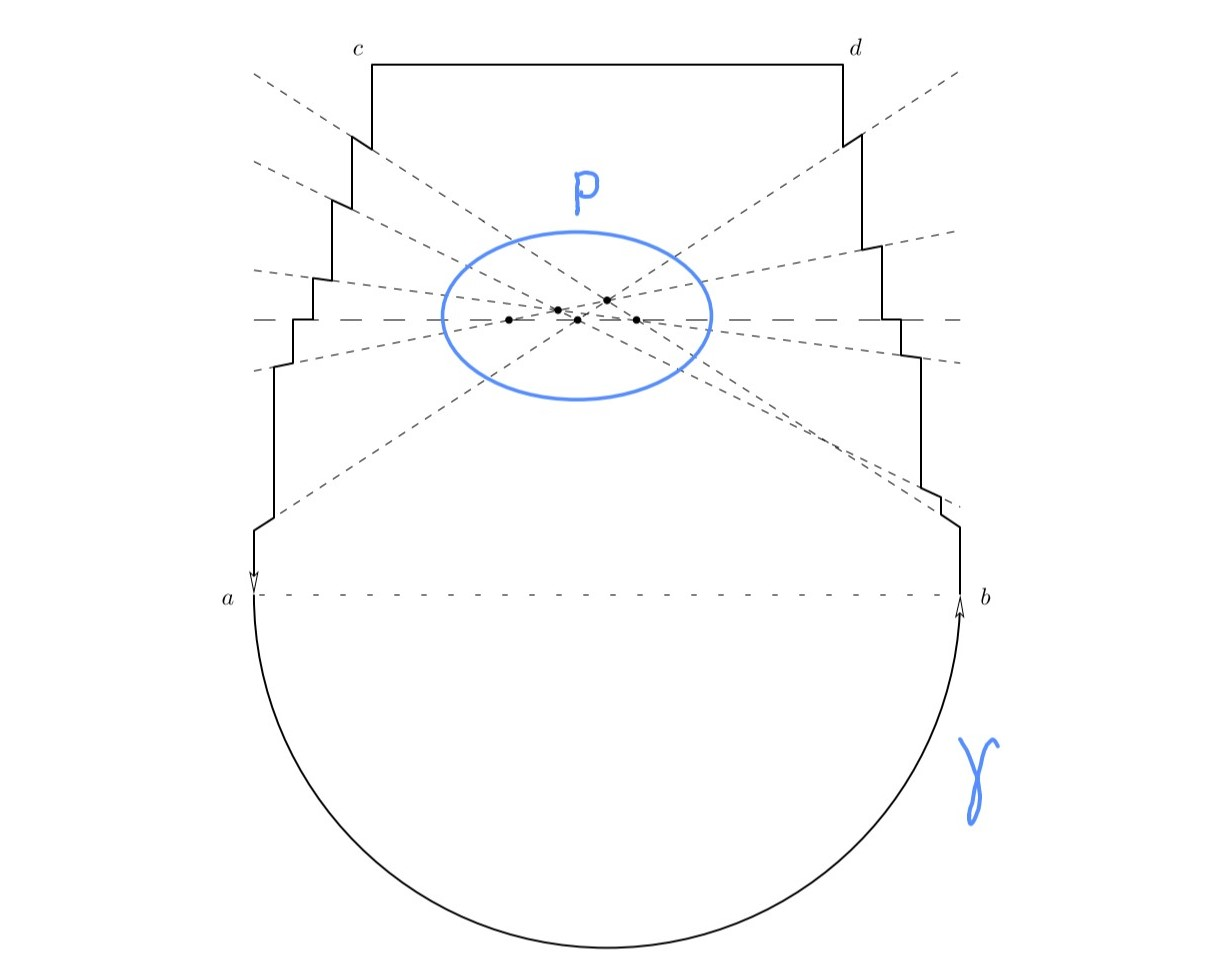
\includegraphics[width=250pt]{grafiken/wenigerkrumm-np1.jpg}
    \caption{Konstruktion der Kurve $\gamma$ (übernommen von \cite{nphard}).}
\end{figure}

Anschließend wird jede Ecke in $\gamma$ abgerundet, indem $2|L_p| + 2(|L_P| + 1) + 1$ neue Punkte auf einem Kreissegment eingefügt werden, wie in Abbildung 2 zu sehen. Daneben werden $n$ Punkte auf jedem Liniensegment von $\gamma$ eingefügt (nicht ausgefüllt in Abbildung 2).

\begin{figure}[h]
    \centering
    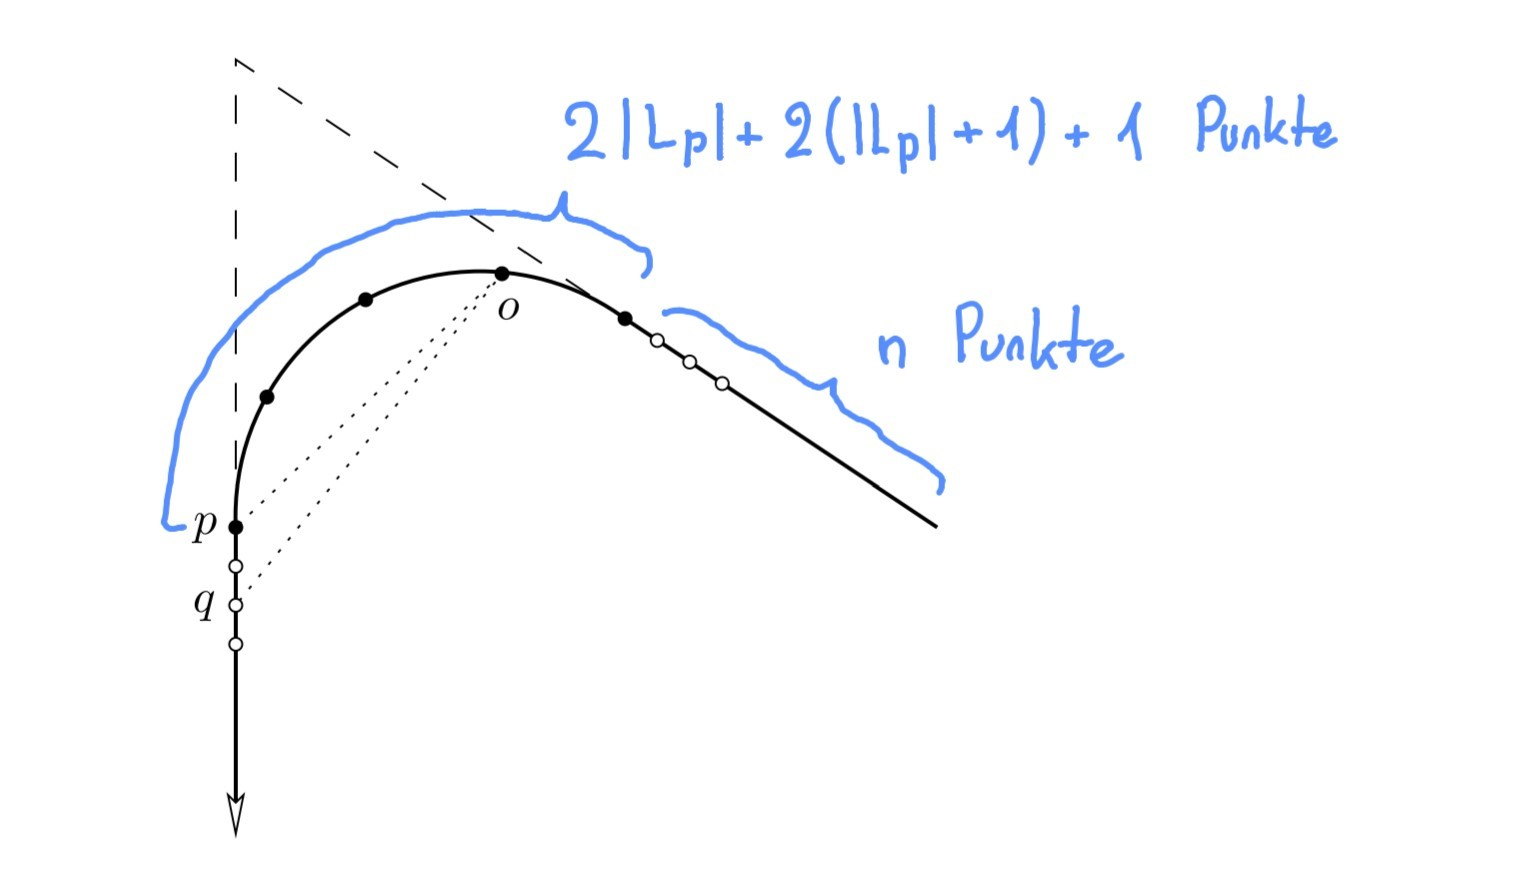
\includegraphics[width=250pt]{grafiken/wenigerkrumm-np2.jpg}
    \caption{Abrundung der Ecken von $\gamma$ (übernommen von \cite{nphard}).}
\end{figure}

 Die Punktemenge $Q$, die Eingabe für \emph{Angle-bounded Hamiltonian Path} ist, besteht aus $P$, den Punkten auf den Kreissegmenten und den jeweils $n$ Punkten auf den Liniensegmenten. In \cite{nphard} wurde für $Q$ Folgendes bewiesen.

\begin{enumerate}
    \item Wenn es $k$ Geraden gibt ($k \le n)$, die die Punkte aus $P$ abdecken, dann gibt es einen Hamiltonzyklus in $Q$ mit Abbiegewinkeln kleiner gleich $(k + 2)\theta$.
    \item Wenn es einen Hamiltonzyklus in $Q$ mit Abbiegewinkeln kleiner gleich $k\theta$ gibt ($k \le n)$, dann gibt es $k$ Geraden, die alle Punkte in $P$ abdecken. 
\end{enumerate}

$\theta$ ist definiert als $\pi / t$, wobei $t = \lceil 9 n^2 \pi / \alpha \rceil$, und $\alpha = \alpha_P / n^\mu$ \cite{nphard}. $\alpha_P$ ist der kleinste Winkel zwischen zwei unterschiedlichen Geraden aus $L_P$, und $\mu$ eine Konstante $\ge 1$. Die genaue Definition ist aber nicht wichtig für die Anpassung des Beweises für Hamiltonpfade. Aus 1. folgt direkt, dass es einen Hamiltonpfad mit Abbiegewinkeln kleiner gleich $(k + 2)\theta$ in $Q$ gibt, denn eine Kante des Hamiltonzyklus kann einfach weggelassen werden. Bezüglich 2. wurde in \cite{nphard} der Hamiltonzyklus in $Q$ in mehrere Runden aufgeteilt, wobei eine Runde aus einigen Punkten im Halbkreis von $a$ zu $b$ (siehe Abbildung 1), und einigen Punkten auf der rechten und linken Seite besteht. In einer Runde kann der Zyklus maximal eine Abkürzung über Punkte aus $P$ verwenden, und die dabei besuchten Punkte aus $P$ müssen immer kolinear sein. Andernfalls würde die Einschränkung des Abbiegewinkels nicht eingehalten werden \cite{nphard}. Anschließend wird in \cite{nphard} gezeigt, dass es maximal $k$ Runden gibt, woraus direkt folgt, dass sich die Punkte aus $P$ mit $k$ Geraden abdecken lassen, da in jeder Runde höchstens eine Abkürzung verwendet wird, und eine Abkürzung einer Geraden zugeordnet werden kann. Auch den Hamiltonpfad kann man in Runden aufteilen, und der Beweis, dass es in ihm höchstens $k$ Runden gibt, ist identisch zu dem für den Hamiltonzyklus in \cite{nphard}. Nun gibt es zwei Fälle: Keiner der Endpunkte des Hamiltonpfads liegt in $P$ oder mindestens einer. Im ersten Fall folgt, dass es $k$ Geraden gibt, die die Punkte von $P$ abdecken, da jeder Runde maximal eine Gerade zugeordnet werden kann (gleiches Argument wie oben). Im zweiten Fall kann der Pfad in der ersten bzw. letzten Runde zweimal Punkte aus $P$ besuchen, wie in Abbildung 3 veranschaulicht. Es folgt, dass es $k + 1$ Geraden gibt, die die Punkte aus $P$ abdecken. Das zeigt, dass \emph{Angle-bounded Hamiltonian Path} (und damit das vorliegende Problem) NP-schwer ist. Denn könnte man effizient bestimmen, ob es einen Hamiltonpfad in $Q$ mit Abbiegewinkeln kleiner gleich $k \theta$ gibt, könnte man effizient bestimmen, ob $P$ mit $k + 1$ Geraden abdeckbar ist. Der Beweis zeigt, dass bereits das Finden eines Hamiltonpfads mit Einschränkung des Abbiegewinkels NP-schwer ist, ohne die Minimierung der Länge.

\begin{figure}[h]
    \centering
    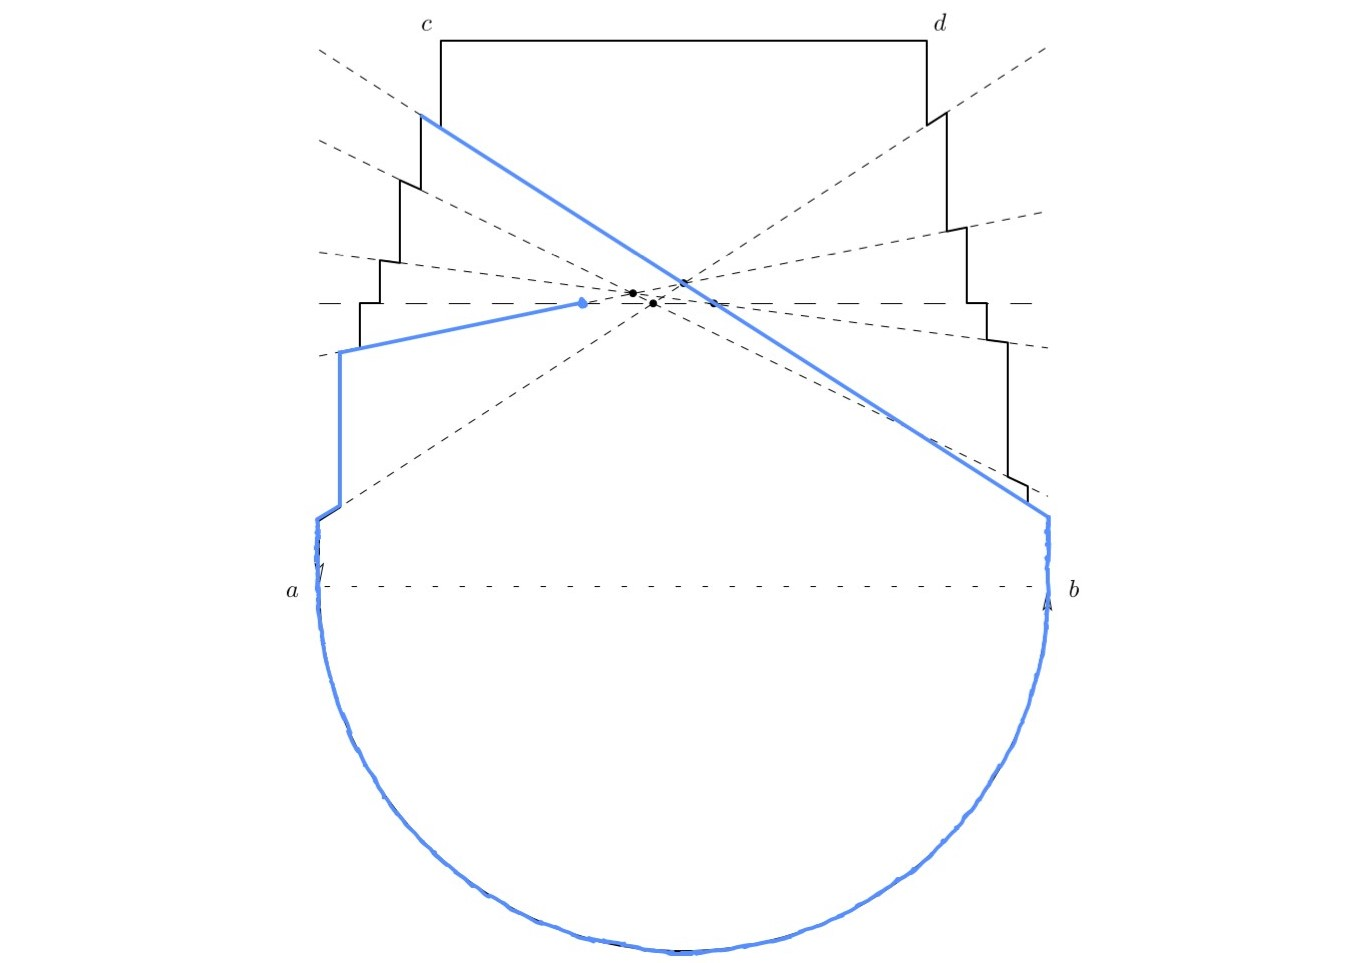
\includegraphics[width=250pt]{grafiken/wenigerkrumm-np3.jpg}
    \caption{Bei einem Hamiltonpfad können in der ersten oder letzten Runde zweimal Punkte aus $P$ besucht werden (übernommen von \cite{nphard}).}
\end{figure}

\section{Laufzeitanalyse}

Um die Laufzeit des Ansatzes zu charakterisieren, soll die Größe des IP in Abhängigkeit von $n$, der Anzahl an Knoten analysiert werden. Da es für jedes unterschiedliche Paar an Knoten eine Variable $x_{ij}$ gibt, ist die Anzahl an Variablen $\binom n 2 = n(n - 1) / 2 = \Theta(n^2)$. Im Folgenden wird die Anzahl an Bedingungen in den Gleichungen (2) - (6) analysiert.

Von (2) und (3) werden jeweils $n$ Bedingungen in das IP eingefügt. Gleichung (4) trägt eine Bedingung bei, sodass Gleichungen (2) - (4) insgesamt $\Theta(n)$ Bedingungen beitragen. Von Ungleichung (5) wird im schlechtesten Fall eine Bedingung für jede nichtleere Teilmenge von $V$ eingefügt, was zu $O(2^n)$ Bedingungen führt. Die genaue Anzahl an Bedingungen von (6) hängt von der gegebenen Instanz ab. Wie bereits angemerkt wurde, werden für jedes ungeordnete Tripel an Punkten, von denen es $\Theta(n^3)$ gibt, 2 oder 3 Bedingungen eingefügt, insgesamt also $\Theta(n^3)$ Bedingungen. Das ganzzahlige lineare Programm in (1) - (7) hat also $\Omega(n^3)$ und $O(2^n + n^3)$ Bedingungen.

Die Lösung eines ganzzahligen linearen Programms ist NP-schwer und benötigt im schlechtesten Fall exponentielle Zeit in der Anzahl an Variablen. Die Laufzeit einer einzigen Lösung ist also exponentiell in $n(n-1)/2$. Durch das allmähliche Hinzufügen von SECs wird das IP mehrmals gelöst, im schlechtesten Fall $O(2^n)$ mal. Die Laufzeit bleibt dadurch immer noch exponentiell. Eine genauere Charakterisierung als ,,exponentiell'' ist nicht wirklich sinnvoll, da dafür Details des IP-Solvers einbezogen werden müssten.

\section{Implementierung}

Das Programm wird in C++ geschrieben und wurde auf Linux-Systemen getestet. Als IP-Solver wird der Open-Source Solver HiGHS verwendet \cite{highs}. Zum Ausführen des Programms muss dieser installiert werden, eine Anleitung dazu findet sich in der \href{https://ergo-code.github.io/HiGHS/dev/cpp/get-started/}{Dokumentation von HiGHS}. Zum Kompilieren kann im Order \verb|aufgabe1| einfach \verb|make| im Terminal ausgeführt werden. Um das Programm z. b. auf \verb|wenigerkrumm1| auszuführen kann im Ordner \verb|aufgabe1|

\medskip
\verb|./aufgabe1 < beispiele/wenigerkrumm1.txt|
\medskip

\noindent ausgeführt werden. Ausgegeben wird die Tourlänge sowie die Punkte in der Reihenfolge der gefundenen Lösung.

Bei der Installation von HiGHS trat auf meinem PC ein Problem auf, dessen Lösung kurz beschrieben wird. Bei der Installation nach der \href{https://ergo-code.github.io/HiGHS/dev/cpp/get-started/}{Anleitung in der Dokumentation} wurden die Headerdateien von HiGHS in \verb|/usr/local/include/highs/| gespeichert. Damit der Compiler eine Headerdatei findet, muss sie aber in \verb|/usr/local/include/| liegen. Damit der Include \verb|#include "Highs.h"| funktioniert, musste ich alle Dateien in \verb|/usr/local/include/highs/| nach \verb|/usr/local/include/| verschieben. Möglicherweise ist das auf anderen PCs auch nötig.

Einen Überblick über HiGHS verschafft \href{https://ergo-code.github.io/HiGHS/dev/cpp/library/}{dieses Beispiel}. Da aber noch keine ausführliche Dokumentation verfügbar ist, wird das Wichtigste hier kurz erklärt. Das ganzzahlige lineare Programm wird in ein \verb|HighsModel| geschrieben, das dann an ein Objekt der Klasse \verb|Highs| gegeben wird. \verb|HighsModel| besitzt das Attribut \verb|lp_|, in dem sich alle relevanten Datenstrukturen zur Spezifizierung des IP befinden. Die folgende Beschreibung bezieht sich auf die Attribute von \verb|lp_|. Die Bedingungsmatrix \verb|a_matrix_| ist eine dünnbesetzte Matrix, in der alle Einträge, die nicht 0 sind, in einem einzigen Vektor \verb|a_matrix_.value_| nach Zeile geordnet gespeichert werden. Die Spaltenindizes der Einträge stehen in \verb|a_matrix_.index_|. Eine Zeile nimmt immer einen kontinuierlichen Bereich in \verb|a_matrix_.value_| bzw. \verb|a_matrix_.index_| ein. Der Index des ersten Eintrags jeder Zeile steht in \verb|a_matrix_.start_|. Das bedeutet, \verb|a_matrix_.start_| wird zu Beginn auf \verb|{0}| gesetzt. Dann wird eine neue Zeile hinzugefügt, indem ihre Indizes und Koeffizienten an \verb|a_matrix_.index_| und \verb|a_matrix.value_| angefügt werden. Die neue Länge von \verb|a_matrix_.index_| bzw. \verb|a_matrix_.value_| wird der Index des ersten Elements der nächsten hinzugefügten Zeile sein, daher wird sie an \verb|a_matrix_.start_| angefügt. \verb|row_lower_| und \verb|row_upper_| speichern die Unter- und Oberschranke für den Wert jeder Zeile, \verb|col_lower_| und \verb|col_upper_| für jede Spalte. Beim Einfügen einer neuen Zeile werden Unter- und Oberschranke der Zeile jeweils an \verb|row_lower_| bzw. \verb|row_upper_| angefügt. \verb|col_cost_| speichert die Koeffizienten der Kostenfunktion. Der Vektor \verb|integrality_| enthält den Typ jeder Variablen (ob ganzzahlig oder reel).

Es erweist sich als praktisch, Punkte im zweidimensionalen Raum als komplexe Zahlen \verb|complex<double>| zu repräsentieren, d. h. die $x$-Koordinate entspricht dem Realteil und $y$-Koordinate dem Imaginärteil. 

\subsection{nchoose2}
\verb|size_t nchoose2(size_t n)|
\medskip

\noindent Gibt $\binom n 2$ zurück.

\subsection{edge\_index}

\verb|size_t edge_index(size_t n, size_t i, size_t j)|
\medskip

\noindent Gibt den Index der zur Kante $\{i, j\}$ zugehörigen Variable $x_{ij}$ zurück. Die Variablen $x_{ij}$ für $i < j$ werden lexikographisch nummeriert, das heißt $x_{01}$ hat Index 0, $x_{02}$ Index 1, \dots, $x_{12}$ Index $n - 1$, $x_{23}$ Index $n - 1 + n - 2$ und so weiter. Der Term $\binom n 2 - \binom {n - \min(i, j)} 2$ gibt den Anfang des ,,Blocks'' von $\min(i, j)$ an, und $\max(i, j) - \min(i, j) - 1$ den Index innerhalb des Blocks.

\subsection{dot\_product}
\verb|double dot_product(complex<double> const &a, complex<double> const &b)|
\medskip

\noindent Gibt das Skalarprodukt von $a$ und $b$, als Vektoren interpretiert, zurück. Es entspricht dem Realteil von $a \bar b$, da $a \bar b = a_1 b_1 + a_2 b_2 - a_1 b_2 i + a_2 b_1 i$, wenn $a = a_1 + a_2 i, b = b_1 + b_2 i$.

\subsection{add\_angle\_constraints}
\verb|void add_angle_constraints(| \\
\verb|    HighsModel &model, vector<complex<double>> const &z)|
\medskip

\noindent Fügt die in Ungleichung (6) bestimmten Bedingungen zu \verb|model| hinzu. Dazu wird über jeden möglichen Scheitelpunkt ($j$) und alle unterschiedlichen Knotenpaare $i, k$ mit $i \ne j \ne k$ und $i < k$ iteriert. Wenn der Winkel $ijk$ spitz ist, werden die Variablen von $\{i, j\}$ und $\{j, k\}$ zu einer neuen Zeile hinzugefügt und ihre Koeffizienten auf 1 gesetzt. Die Unterschranke für die neue Zeile der Matrix ist 0, die Oberschranke 1.

\subsection{add\_degree\_constraints}
\verb|void add_degree_constraints(HighsModel &model, size_t n)|
\medskip

\noindent Fügt für jeden Knoten $i$ eine Zeile in die Bedingungsmatrix ein, in der die Variablen aller Kanten aufsummiert werden, von denen $i$ ein Endpunkt ist. Der Wert der Zeile wird auf $[1, 2]$ beschränkt, womit Ungleichungen (2) und (3) umgesetzt werden.

\subsection{add\_num\_edges\_constraint}
\verb|void add_num_edges_constraint(HighsModel &model, size_t n)|
\medskip

\noindent Beschränkt die Anzahl verwendeter Kanten auf genau $n - 1$, indem alle $\binom n 2$ Variablen in einer neuen Zeile aufsummiert werden, und der Wert der Zeile auf $n - 1$ fixiert wird.

\subsection{add\_subtour\_elimination\_constraint}
\verb|void add_subtour_elimination_constraint(| \\
\verb|    Highs &highs, size_t n, vector<size_t> const &tour)|
\medskip

\noindent Fügt für die Knoten in \verb|tour| einen Subtour Elimination Constraint ein, wie in Ungleichung (5) beschrieben. Da diese Funktion nach nach Übergabe des \verb|HighsModel| an das \verb|Highs|-Objekt verwendet wird, wird die Funktion \verb|Highs::addRow| verwendet. Ihre Parameter sind die Unterschranke und Oberschranke der neuen Zeile, die Anzahl an Einträgen, die nicht 0 sind, und Zeiger zu den Indizes und Werten. Zuerst werden zwei Arrays \verb|ind| und \verb|val| angelegt. Da in der neuen Zeile die Variablen für jede Kante zwischen zwei Knoten in \verb|tour| aufsummiert werden sollen, wird über jedes Paar an Knoten in \verb|tour| iteriert. Der Index der Kante zwischen dem Paar wird in \verb|ind| eingefügt und der Koeffizient in \verb|val| auf 1 gesetzt. Schließlich wird \verb|Highs::addRow| aufgerufen und die Oberschranke der neuen Zeile auf \verb|tour.size() - 1| gesetzt.

\subsection{build\_graph}
\verb|vector<vector<size_t>> build_graph(Highs const &highs, size_t n)|
\medskip

\noindent Gibt den Graphen in Form einer Adjazenzliste zurück, der genau die Kanten aus der in \verb|highs| gespeicherten Lösung enthält. Dazu wird über jedes Knotenpaar $i, j$ mit $i < j$ iteriert, und wenn der Wert der zu $\{i, j\}$ zugehörigen Variable 1 ist, wird die Kante $\{i, j\}$ in den Graphen eingefügt. Da die Variablen in der Lösung nur 0 oder 1 sein können aber aufgrund von Rundungsfehlern möglicherweise nicht exakt 0 oder 1 sind, wird die Bedingung \verb|> 0.5| anstatt \verb|== 1| verwendet.

\subsection{check\_for\_subtours}
\verb|bool check_for_subtours(Highs &highs, size_t n)|
\medskip

\noindent Gibt zurück, ob in der in \verb|highs| enthaltenen Lösung Subtouren existieren und eliminiert dies gegebenenfalls. Dafür werden alle Zyklen in dem von \verb|build_graph| erstellten Graphen gefunden. Von jedem noch nicht besuchten Knoten aus wird eine Suche (ähnlich zur Tiefensuche) durchgeführt und festgestellt, ob der Ausgangsknoten \verb|i| wieder erreicht wird. Jeder besuchte Knoten wird als besucht markiert und zu \verb|subtour| hinzugefügt. Der Unterschied zur Tiefensuche ist, dass immer nur ein Nachbar betrachtet wird, was ausreicht, da jeder Knoten maximal Grad 2 hat. Wird \verb|i| wieder erreicht, enthält \verb|subtour| den gesamten Zyklus, von dem \verb|i| Teil ist, und es wird ein Subtour Elimination Constraint für ihn hinzugefügt.

\subsection{get\_optimal\_tour}

\verb|pair<vector<complex<double>>, double> get_optimal_tour(| \\
\verb|    vector<complex<double>> const &z)|
\medskip

\noindent Gibt den kürzesten Hamiltonpfad mit Abbiegewinkeln von maximal $\pi / 2$ als Permutation der in \verb|z| gegebenen Punkte zurück, sowie dessen Länge. Falls keine Lösung existiert, wird ein leerer Vektor zurückgegeben.

Zunächst werden grundsätzliche Eigenschaften des \verb|model| festgelegt, z. B. dass die Zielfunktion minimiert werden soll und die Anzahl an Spalten oder Variablen $\binom n 2$ ist. Darauf wird über jedes Knotenpaar $i, j$ mit $i < j$ iteriert und der Koeffizient der Variable $x_{ij}$ auf $d_{ij}$ gesetzt. Daneben wird festgelegt, dass $x_{ij} \in \{0, 1\}$ sein muss. Anschließend werden die verschiedenen Bedingungen zu \verb|model| hinzugefügt und dessen Anzahl an Zeilen aktualisiert.

Danach wird das Objekt \verb|highs| angelegt und ihm \verb|model| übergeben. Solange Subtouren existieren und nicht festgestellt wurde, dass es keine Lösung gibt (signalisiert durch \verb|HighsModelStatus::kInfeasible|), wird das IP mit \verb|Highs::run| gelöst und entsprechende SECs eingefügt.

Falls eine Lösung existiert, wird der Graph mit Kanten aus der Lösung mithilfe von \verb|build_graph| erstellt. Anschließend wird ein Knoten mit Grad 1 als Startpunkt für eine Suche durch den Graphen ausgewählt. Die Suche zum Finden des Hamiltonpfads funktioniert wie in \verb|check_for_subtours|, es wird immer ein aktueller Knoten \verb|j| und dessen Vorgänger \verb|last| verwaltet. Jeder besuchte Knoten wird zum Vektor \verb|tour| hinzugefügt, der am Ende zurückgegeben wird.

\section{Beispiele}

Die Instanzen von BWINF konnten alle optimal gelöst werden. Für die größte von ihnen, \emph{wenigerkrumm3} mit 120 Punkten, wurde 1 min 4,14 s benötigt. Die Laufzeitmessungen wurden mit einem AMD Ryzen 5 3600 durchgeführt, es standen 15,6 GB Arbeitsspeicher zur Verfügung. Alle Beispiele nach \emph{wenigerkrumm8} stammen von TSPLIB \cite{tsplib}, allerdings wurden die Eingabedateien vom TSPLIB-Format in das Format der anderen Eingaben umgewandelt. Für die BWINF-Instanzen waren maximal 6 SECs nötig, was die obige Begründung für die DFJ-Formulierung unterstützt. Mit 29 SECs waren bei der TSPLIB-Instanz a280 die meisten SECs nötig, was im Verhältnis zu den 280 Punkten dieser Instanz aber immer noch wenig ist. Die Zahl an Bedingungen der ganzzahligen linearen Programme wurde stets von den $\Theta(n^3)$ Winkelbedingungen dominiert. Die größte gelöste Instanz von TSPLIB (lin318) bestand aus 318 Punkten und benötigte ca. 30 min. Da die Programmausgaben viel Platz benötigen, sind die Ausgaben für die BWINF-Beispiele im Anhang zu finden. Die Lösungen werden hier graphisch präsentiert. Die Ausgaben für alle Beispiele finden sich im Ordner \verb|ausgaben|.

\subsection{wenigerkrumm1}

\includesvg[width=398pt]{grafiken/wenigerkrumm1}

\noindent Tourlänge: 847.434165 $\quad$ Laufzeit: 0,607 s $\quad$ \#SECs: 0

\subsection{wenigerkrumm2}

\includesvg[width=398pt]{grafiken/wenigerkrumm2}

\noindent Tourlänge: 2183.662266 $\quad$ Laufzeit: 2,935 s $\quad$ \#SECs: 2

\subsection{wenigerkrumm3}

\includesvg[width=398pt]{grafiken/wenigerkrumm3}

\noindent Tourlänge: 1848.046986 $\quad$ Laufzeit: 1 min 4,14 s $\quad$ \#SECs: 6

\subsection{wenigerkrumm4}

\includesvg[width=398pt]{grafiken/wenigerkrumm4}

\noindent Tourlänge: 1205.068555 $\quad$ Laufzeit: 0,024 s $\quad$ \#SECs: 0

\subsection{wenigerkrumm5}

\includesvg[width=398pt]{grafiken/wenigerkrumm5}

\noindent Tourlänge: 3257.920434 $\quad$ Laufzeit: 0,375 s $\quad$ \#SECs: 0
\medskip

\noindent Eine bemerkenswerte Eigenschaft der optimalen Lösungen ist, dass sie sich selbst schneiden können. Bei optimalen Lösungen des TSP auf euklidschen Graphen ist das nicht möglich. 

\subsection{wenigerkrumm6}

\includesvg[width=398pt]{grafiken/wenigerkrumm6}

\noindent Tourlänge: 3457.994092 $\quad$ Laufzeit: 22,35 s $\quad$ \#SECs: 2

\subsection{wenigerkrumm7}

\includesvg[width=398pt]{grafiken/wenigerkrumm7}

\noindent Tourlänge: 4150.643872 $\quad$ Laufzeit: 17,83 s $\quad$ \#SECs: 3

\subsection{wenigerkrumm8}

Dieses Beispiel (ein Dreieck mit keinem Winkel größer gleich $\pi / 2$) zeigt, dass das Programm erkennt, wenn keine Tour möglich ist.
\medskip

\noindent Eingabe:
\begin{verbatim}
0.0 0.0
6.0 0.0
3.0 5.0
\end{verbatim}

\noindent Ausgabe:
\begin{verbatim}
Keine Tour mit maximalem Abbiegewinkel von 90 Grad möglich.
\end{verbatim}

\subsection{a280}

\includesvg[width=398pt]{grafiken/a280}

\noindent Tourlänge: 2753.696953 $\quad$ Laufzeit: 26 m 3 s $\quad$ \#SECs: 29

\subsection{berlin52}

\includesvg[width=398pt]{grafiken/berlin52}

\noindent Tourlänge: 9311.526799 $\quad$ Laufzeit: 3,908 s $\quad$ \#SECs: 0

\subsection{ch130}

\includesvg[width=398pt]{grafiken/ch130}

\noindent Tourlänge: 7365.270508 $\quad$ Laufzeit: 1 min 51 s $\quad$ \#SECs: 5

\subsection{kroA100}

\includesvg[width=398pt]{grafiken/kroA100}

\noindent Tourlänge: 28421.204198 $\quad$ Laufzeit: 25,35 s $\quad$ \#SECs: 2 

\subsection{kroA200}

\includesvg[width=398pt]{grafiken/kroA200}

\noindent Tourlänge: 37365.104952 $\quad$ Laufzeit: 17 m 4 s $\quad$ \#SECs: 5 

\subsection{kroB100}

\includesvg[width=398pt]{grafiken/kroB100}

\noindent Tourlänge: 26943.309447 $\quad$ Laufzeit: 23,48 s $\quad$ \#SECs: 3 

\subsection{kroB150}

\includesvg[width=398pt]{grafiken/kroB150}

\noindent Tourlänge: 31214.645516 $\quad$ Laufzeit: 3 m 33 s $\quad$ \#SECs: 8

\subsection{kroB200}

\includesvg[width=398pt]{grafiken/kroB200}

\noindent Tourlänge: 35061.000654 $\quad$ Laufzeit: 23 m 35 s $\quad$ \#SECs: 4 

\subsection{lin318}

\includesvg[width=398pt]{grafiken/lin318}

\noindent Tourlänge: 51648.008358 $\quad$ Laufzeit: 30 min 29 s $\quad$ \#SECs: 4

\subsection{pr299}

\includesvg[width=398pt]{grafiken/pr299}

\noindent Tourlänge: 56257.537596 $\quad$ Laufzeit: 50 m 59 s $\quad$ \#SECs: 18

\subsection{tsp225}

\includesvg[width=398pt]{grafiken/tsp225}

\noindent Tourlänge: 3805.926070 $\quad$ Laufzeit: 54,18 s $\quad$ \#SECs: 1
\medskip

\noindent Die Form der Tour lässt vermuten, dass die Lösung nahezu mit der optimalen Lösung für das TSP übereinstimmt.

\section{Quellcode}

\subsection{util.hpp}

\inputminted{c++}{aufgabe1/util.hpp}

\subsection{aufgabe1\_ip.cpp}

\inputminted{c++}{aufgabe1/aufgabe1_ip.cpp}

\subsection{aufgabe1\_randomized.cpp}

\inputminted{c++}{aufgabe1/aufgabe1_randomized.cpp}

\begin{thebibliography}{4}
    \bibitem{tsp-formulations}
    Öncan, T., Altinel, I. K., Laporte, G. (2009).
    A comparative analysis of several asymmetric traveling salesman problem formulations. \\
    \href{https://mate.unipv.it/gualandi/famo2conti/papers/tsp_formulations.pdf}{https://mate.unipv.it/\textasciitilde{}gualandi/famo2conti/papers/tsp\_formulations.pdf}
    
    \bibitem{highs}
    Huangfu, Q., Hall, J. A. J. (2018).
    Parallelizing the dual revised simplex method. \\
    \href{https://www.maths.ed.ac.uk/hall/HuHa13/}{https://www.maths.ed.ac.uk/hall/HuHa13/} \\
    \href{https://github.com/ERGO-Code/HiGHS}{https://github.com/ERGO-Code/HiGHS}

    \bibitem{tsplib}
    Ruprecht-Karls Universität Heidelberg. TSPLIB \\
    \href{http://comopt.ifi.uni-heidelberg.de/software/TSPLIB95/}{http://comopt.ifi.uni-heidelberg.de/software/TSPLIB95/}

    \bibitem{nphard}
    Dumitrescu, A., Jiang, M. (2018).
    On the approximability of covering points by lines and related problems. \\
    \href{https://arxiv.org/pdf/1312.2549.pdf}{https://arxiv.org/pdf/1312.2549.pdf}

    \bibitem{discrete-math}
    Johnsonbaugh, R. (2018). 
    Discrete Mathematics (Eighth Edition).
\end{thebibliography}

\section*{Anhang}
\addcontentsline{toc}{section}{Anhang}

\subsection*{wenigerkrumm1}

\begin{verbatim}
Tourlänge: 847.434165
400.000000 30.000000
390.000000 30.000000
380.000000 30.000000
370.000000 30.000000
360.000000 30.000000
350.000000 30.000000
340.000000 30.000000
330.000000 30.000000
320.000000 30.000000
310.000000 30.000000
300.000000 30.000000
290.000000 30.000000
280.000000 30.000000
270.000000 30.000000
260.000000 30.000000
250.000000 30.000000
240.000000 30.000000
230.000000 30.000000
220.000000 30.000000
210.000000 30.000000
200.000000 30.000000
190.000000 30.000000
180.000000 30.000000
170.000000 30.000000
160.000000 30.000000
150.000000 30.000000
140.000000 30.000000
130.000000 30.000000
120.000000 30.000000
110.000000 30.000000
100.000000 30.000000
90.000000 30.000000
80.000000 30.000000
70.000000 30.000000
60.000000 30.000000
50.000000 30.000000
40.000000 30.000000
30.000000 30.000000
20.000000 30.000000
10.000000 30.000000
0.000000 30.000000
-5.000000 15.000000
0.000000 0.000000
10.000000 0.000000
20.000000 0.000000
30.000000 0.000000
40.000000 0.000000
50.000000 0.000000
60.000000 0.000000
70.000000 0.000000
80.000000 0.000000
90.000000 0.000000
100.000000 0.000000
110.000000 0.000000
120.000000 0.000000
130.000000 0.000000
140.000000 0.000000
150.000000 0.000000
160.000000 0.000000
170.000000 0.000000
180.000000 0.000000
190.000000 0.000000
200.000000 0.000000
210.000000 0.000000
220.000000 0.000000
230.000000 0.000000
240.000000 0.000000
250.000000 0.000000
260.000000 0.000000
270.000000 0.000000
280.000000 0.000000
290.000000 0.000000
300.000000 0.000000
310.000000 0.000000
320.000000 0.000000
330.000000 0.000000
340.000000 0.000000
350.000000 0.000000
360.000000 0.000000
370.000000 0.000000
380.000000 0.000000
390.000000 0.000000
400.000000 0.000000
405.000000 15.000000
\end{verbatim}

\subsection*{wenigerkrumm2}

\begin{verbatim}
Tourlänge: 2183.662266
-88.167788 121.352549
-111.471724 100.369591
-129.903811 75.000000
-142.658477 46.352549
-149.178284 15.679269
-149.178284 -15.679269
-142.658477 -46.352549
-129.903811 -75.000000
-111.471724 -100.369591
-88.167788 -121.352549
-61.010496 -137.031819
-31.186754 -146.722140
0.000000 -150.000000
31.186754 -146.722140
61.010496 -137.031819
88.167788 -121.352549
111.471724 -100.369591
129.903811 -75.000000
142.658477 -46.352549
149.178284 -15.679269
149.178284 15.679269
142.658477 46.352549
129.903811 75.000000
111.471724 100.369591
88.167788 121.352549
61.010496 137.031819
31.186754 146.722140
0.000000 150.000000
-31.186754 146.722140
-61.010496 137.031819
-117.557050 161.803399
-148.628965 133.826121
-173.205081 100.000000
-190.211303 61.803399
-198.904379 20.905693
-198.904379 -20.905693
-190.211303 -61.803399
-173.205081 -100.000000
-148.628965 -133.826121
-117.557050 -161.803399
-81.347329 -182.709092
-41.582338 -195.629520
0.000000 -200.000000
41.582338 -195.629520
81.347329 -182.709092
117.557050 -161.803399
148.628965 -133.826121
173.205081 -100.000000
190.211303 -61.803399
198.904379 -20.905693
198.904379 20.905693
190.211303 61.803399
173.205081 100.000000
148.628965 133.826121
117.557050 161.803399
81.347329 182.709092
41.582338 195.629520
0.000000 200.000000
-41.582338 195.629520
-81.347329 182.709092 
\end{verbatim}

\subsection*{wenigerkrumm3}

\begin{verbatim}
Tourlänge: 1848.046986
0.000000 20.000000
-16.632935 21.748192
-32.538931 26.916363
-47.022820 35.278640
-59.451586 46.469551
-69.282032 40.000000
-76.084521 24.721360
-79.561752 8.362277
-79.561752 -8.362277
-76.084521 -24.721360
-69.282032 -40.000000
-59.451586 -53.530449
-47.022820 -64.721360
-32.538931 -73.083637
-16.632935 -78.251808
0.000000 -80.000000
16.632935 -78.251808
32.538931 -73.083637
47.022820 -64.721360
52.977180 -64.721360
67.461069 -73.083637
83.367065 -78.251808
100.000000 -80.000000
116.632935 -78.251808
132.538931 -73.083637
147.022820 -64.721360
159.451586 -53.530449
169.282032 -40.000000
176.084521 -24.721360
179.561752 -8.362277
179.561752 8.362277
176.084521 24.721360
169.282032 40.000000
159.451586 46.469551
147.022820 35.278640
132.538931 26.916363
116.632935 21.748192
100.000000 20.000000
83.367065 21.748192
76.084521 24.721360
69.282032 40.000000
59.451586 46.469551
59.451586 53.530449
69.282032 60.000000
76.084521 75.278640
83.367065 78.251808
100.000000 80.000000
116.632935 78.251808
132.538931 73.083637
147.022820 64.721360
159.451586 53.530449
169.282032 60.000000
176.084521 75.278640
179.561752 91.637723
179.561752 108.362277
176.084521 124.721360
169.282032 140.000000
159.451586 153.530449
147.022820 164.721360
132.538931 173.083637
116.632935 178.251808
100.000000 180.000000
83.367065 178.251808
67.461069 173.083637
52.977180 164.721360
47.022820 164.721360
32.538931 173.083637
16.632935 178.251808
0.000000 180.000000
-16.632935 178.251808
-32.538931 173.083637
-47.022820 164.721360
-59.451586 153.530449
-69.282032 140.000000
-76.084521 124.721360
-79.561752 108.362277
-79.561752 91.637723
-76.084521 75.278640
-69.282032 60.000000
-59.451586 53.530449
-47.022820 64.721360
-32.538931 73.083637
-16.632935 78.251808
0.000000 80.000000
16.632935 78.251808
23.915479 75.278640
32.538931 73.083637
30.717968 60.000000
30.717968 40.000000
32.538931 26.916363
23.915479 24.721360
16.632935 21.748192
20.438248 8.362277
20.438248 -8.362277
23.915479 -24.721360
30.717968 -40.000000
40.548414 -53.530449
59.451586 -53.530449
69.282032 -40.000000
76.084521 -24.721360
79.561752 -8.362277
79.561752 8.362277
67.461069 26.916363
52.977180 35.278640
47.022820 35.278640
40.548414 46.469551
40.548414 53.530449
47.022820 64.721360
52.977180 64.721360
67.461069 73.083637
79.561752 91.637723
79.561752 108.362277
76.084521 124.721360
69.282032 140.000000
59.451586 153.530449
40.548414 153.530449
30.717968 140.000000
23.915479 124.721360
20.438248 108.362277
20.438248 91.637723  
\end{verbatim}

\subsection*{wenigerkrumm4}

\begin{verbatim}
Tourlänge: 1205.068555
42.137753 -60.319863
94.789917 -67.087689
144.832862 -43.476284
153.130159 -20.360910
139.446709 0.233238
101.498782 33.484198
51.008140 5.769601
-16.723130 -12.689542
-20.971208 -5.637107
28.913721 58.699880
33.379688 100.161238
20.212169 156.013261
-107.988514 185.173669
-119.026308 168.453598
-154.088455 115.022553
-219.148505 103.685337
-240.369194 57.426131
-239.414022 40.427118
-239.848226 8.671399
-221.149792 -32.862538
-191.716829 -28.360492
-137.317503 -20.146939
-98.760442 -81.770618
-82.864121 -104.173600
-129.104485 -155.041640
\end{verbatim}

\subsection*{wenigerkrumm5}

\begin{verbatim}
Tourlänge: 3257.920434
267.845908 127.627482
244.228552 119.192512
171.595574 135.520994
116.702667 132.021991
63.541591 55.140221
62.366656 50.713913
45.123674 31.740242
25.098172 35.205544
-8.936916 13.543851
-70.183535 73.738342
-86.457580 105.836348
-82.173510 119.465553
-68.446198 137.178953
27.706327 169.284192
36.599805 147.885350
47.040512 141.206562
51.417675 146.417721
38.654730 188.608557
-30.991436 186.807059
-44.669924 170.088013
-49.447381 173.210759
-104.781549 158.212048
-177.685937 158.265884
-223.039999 171.558368
-258.868593 166.669198
-280.008136 11.657786
-286.024059 -55.955204
-284.547616 -60.154961
-278.409792 -111.914073
-281.678990 -187.717923
-260.477802 -196.955535
-251.656688 -195.189953
-214.362324 -193.265190
-116.831788 -191.380552
-41.263039 -144.118212
-57.266232 -115.737582
-58.684205 -76.988884
-31.548604 -55.223912
-74.639411 25.542881
-81.384378 32.368323
-95.621797 77.468533
-136.787038 79.501703
-235.099412 47.810306
-247.341131 -160.277639
-234.711279 -162.774591
-202.218443 -178.735864
-147.023475 -166.220130
26.451074 -192.813352
30.366828 -167.573232
90.584569 -164.218416
142.765554 -118.682439
162.493244 -84.574019
141.513053 2.821137
92.639946 22.216030
106.033430 69.754891
209.544977 94.267052
239.639550 79.491132
253.534863 38.014987
283.989938 -101.866465
263.236651 -144.293091
\end{verbatim}

\subsection*{wenigerkrumm6}

\begin{verbatim}
Tourlänge: 3457.994092
-288.744132 -173.349893
-293.833463 -165.440105
-189.988471 -98.043874
-144.887799 -73.495410
-126.569816 -30.645224
-139.741580 57.936680
-102.699992 95.632069
-97.391662 124.120512
-167.994506 138.195365
-194.986965 101.363745
-175.118239 77.842636
-100.569041 140.808607
-89.453831 162.237392
-55.091518 198.826966
102.223372 174.201904
154.870684 140.327660
121.661135 85.267672
102.909291 60.107868
83.005905 64.646774
64.559003 82.567627
73.689751 110.224271
85.043830 108.946389
100.006932 76.579303
121.392544 56.694081
81.740403 10.276251
76.647124 -7.289705
112.833346 -38.057607
138.136997 -31.348808
155.341949 -20.252779
172.836936 59.184233
245.415055 44.794067
289.298882 56.051342
277.821597 104.262606
255.134924 115.594915
246.621634 101.705861
231.944823 82.961057
228.929427 82.624982
175.677917 98.929343
151.432196 121.427337
132.794476 135.681392
120.906436 131.798810
96.781707 141.370805
49.091876 150.678826
21.067444 122.164599
20.218290 88.031173
56.716498 66.959624
58.019653 49.937906
58.716620 32.835930
40.327635 19.216022
14.005617 -14.015334
-18.507391 -22.905270
-31.745416 -69.207960
-19.310012 -131.810965
21.176627 -165.421555
46.674278 -193.090008
152.102728 -193.381252
202.346980 -189.069699
242.810288 -182.054289
245.020791 -167.448848
238.583388 -133.143524
210.186432 -127.403563
187.669263 -122.655771
150.526118 -88.230057
134.692592 -102.152826
143.114152 -135.866707
157.588994 -144.200765
216.825920 -152.024123
221.028639 -139.435079
155.405344 -56.437901
92.255820 -93.514104
64.943433 -119.784474
19.765322 -99.236400
-4.590656 -40.067226
-51.343758 -57.654823
-72.565291 -24.281820
-90.160190 -25.200829
-107.196865 -77.792599
-154.225945 -135.522059
-191.216327 -162.689024
-187.485329 -177.031237
\end{verbatim}

\subsection*{wenigerkrumm7}

\begin{verbatim}
Tourlänge: 4150.643872
-181.208895 -192.622935
-202.828627 -101.700050
-172.378071 -88.298187
-152.130365 -93.844349
-133.730932 -113.306155
-155.651746 -138.151811
-189.135201 -139.078513
-244.959501 -111.046573
-217.282470 -43.316616
-211.429137 27.770425
-207.665172 81.410371
-185.649161 90.144456
-189.062172 104.285631
-215.113949 120.740679
-222.492322 169.033315
-240.249363 179.334919
-268.739142 143.276483
-287.058297 113.599823
-284.129027 107.252583
-248.169463 80.132237
-226.787625 2.658862
-184.092700 5.737284
-171.354954 25.463068
-147.363185 59.608175
-126.568914 106.964962
-56.914543 92.501249
-27.911955 48.326745
-42.704691 37.679514
-48.354421 9.091412
-46.403062 -13.755804
-47.266557 -66.984045
-17.356579 -125.254131
34.959132 -106.842499
68.910854 -82.123346
106.599423 -107.433987
126.904044 -80.733297
135.781192 -13.053440
141.433472 -6.023095
129.024315 29.701695
74.887500 80.586458
53.436521 125.683201
54.766523 154.053847
34.079032 187.731112
-13.030259 174.698005
-120.386562 170.589454
-134.985023 132.944989
-157.423365 126.800331
-200.771246 147.741054
-201.485143 155.274830
-192.681053 174.522947
-153.130140 187.817274
-114.146166 190.615321
-84.626900 148.216494
8.643660 135.907430
16.573231 104.020979
40.897139 78.152317
54.551865 71.567133
56.389778 71.618509
57.555364 64.417343
55.434792 62.729160
3.152113 27.103890
-4.434919 33.164884
-18.316063 27.755860
-9.580869 -17.516639
-0.200936 -21.927663
47.011363 -30.887180
55.550895 -45.089968
88.818853 -42.834512
118.989764 -80.203583
172.389228 -53.133270
158.552316 -19.254407
189.387028 -4.465225
239.616628 -21.944160
296.911892 25.811569
271.301094 142.524086
221.808162 186.241012
170.514252 161.169850
169.990437 154.260412
148.108328 123.558283
126.799911 112.727280
120.375033 115.889661
100.043893 161.295125
95.947213 183.278211
130.854855 195.695082
217.218893 164.294928
216.691000 156.314370
208.592696 136.618460
162.923138 117.465744
158.742184 62.618834
178.198360 37.031984
205.717887 -24.976511
224.599361 -34.798485
256.475967 -46.591418
276.276517 -49.448662
278.105364 -93.771765
275.793495 -129.415477
235.827007 -143.838844
217.599278 -189.258062
92.298040 -146.169487
59.827200 -170.713714
\end{verbatim}

\end{document}